\documentclass[pdflatex,12pt]{aghdpl}
%\documentclass{aghdpl}               % przy kompilacji programem latex
% \documentclass[pdflatex,en]{aghdpl}  % praca w języku angielskim
\usepackage[polish]{babel}
\usepackage[utf8]{inputenc}

% dodatkowe pakiety
\usepackage{enumerate}
\usepackage{listings}
\lstloadlanguages{TeX}

\lstset{
  literate={ą}{{\k{a}}}1
           {ć}{{\'c}}1
           {ę}{{\k{e}}}1
           {ó}{{\'o}}1
           {ń}{{\'n}}1
           {ł}{{\l{}}}1
           {ś}{{\'s}}1
           {ź}{{\'z}}1
           {ż}{{\.z}}1
           {Ą}{{\k{A}}}
           {Ć}{{\'C}}1
           {Ę}{{\k{E}}}1
           {Ó}{{\'O}}1
           {Ń}{{\'N}}1
           {Ł}{{\L{}}}1
           {Ś}{{\'S}}1
           {Ź}{{\'Z}}1
           {Ż}{{\.Z}}1
}

%---------------------------------------------------------------------------

\author{Michał Mąka}
\shortauthor{Michał Mąka}

\titlePL{System pomiarów warunków środowiskowych i meteorologicznych}
\titleEN{Measurment system of environmental and weather conditions}

\shorttitlePL{System pomiarów warunków środowiskowych i meteorologicznych} % skrócona wersja tytułu je¶li jest bardzo długi
\shorttitleEN{Measurment system of environmental and weather conditions}

\thesistypePL{Praca inżynierska}
\thesistypeEN{Engineering Thesis}

\supervisorPL{dr inż. Marek Stencel}
\supervisorEN{Marek Stencel Sc.D}

\date{2013}

\departmentPL{Katedra Automatyki i Inżynierii Biomedycznej}
\departmentEN{Department of Automatics and Bioengineering}

\facultyPL{Wydział Elektrotechniki, Automatyki, Informatyki i Inżynierii Biomedycznej}
\facultyEN{Faculty of Electrical Engineering, Automatics, Computer Science and Biomedical Engineering}

\acknowledgements{Podziękowania}



\setlength{\cftsecnumwidth}{10mm}

%---------------------------------------------------------------------------

\begin{document}

\titlepages

\tableofcontents
\clearpage

\addcontentsline{toc}{part}{Wstęp}
\part*{Wstęp}
\chapter*{Wprowadzenie}
\addcontentsline{toc}{chapter}{Wprowadzenie}
\chapter*{Cel i założenia projektu}
\addcontentsline{toc}{chapter}{Cel i założenia projektu}

\part{Część teoretyczna}
\chapter{Komunikacja w układzie}
Magistrala jest to układ linii, po których przekazywane są wszystkie informacje pomiędzy podłączonymi do niej urządzeniami, np. komputerem, czujnikiem, regulatorem itp. Zasada działania magistrali opiera się na uzyskiwaniu oraz nadawaniu współpracującym częściom uprawnień do transmisji danych w danej jednostce czasu. W jednej chwili, w magistrali może działać tylko jedno urządzenie nadające oraz dowolna liczba odbiorców. Systemy o budowie opartej na magistrali są łatwo modyfikowalne oraz rozszerzalne, w prosty sposób można dołączyć lub odłączyć elementy systemu.
Dane przesyłane na dużą odległość najlepiej jest przekazywać transmisją szeregową, na krótsze odległości, przesyłanie równoległe oraz szeregowe daje podobne rezultaty.
Bity oraz całe słowa w tej komunikacji przesyłane są jeden po drugim. Przy takim sposobie łączenia się wystarczą tylko dwa przewody łączące odbiorcę z urządzeniem nadającym. 

Przykład urządzenia w magistrali szeregowej został przedstawiony na poniższym schemacie:
\begin{figure}[h]
\centering
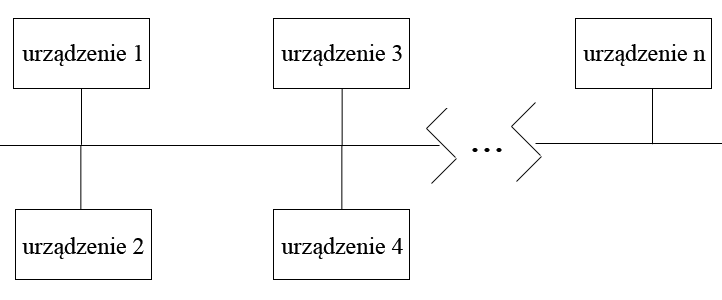
\includegraphics[scale=0.5]{magistrala}
\caption{Schemat magistrali szeregowej}
\label{fig:magistrala}
\end{figure}

Jak widać na załączonym rysunku, można podłączyć do magistrali wiele urządzeń. Wszystkie są podłączone do jednej lini danych, na której odbywa się komunikacja. To właśnie przez nią przesyłane są wszystkie dane pomiędzy elementami magistrali.

\section{Magistrala $\mathbf{I^{2}C}$}
Nazwa jest to akronimem od Inter-Intergrated Circuit. Standard został opracowany w latach osiemdziesiątych przez firmę Philips.

Jest ona bardzo często wykorzystywana w układach mikroprocesorowych, w sterownikach wyświetlaczy LCD, można ją stosować do sterowania pamięci RAM, EPROM, układami I/O.

Zaletami magistrali $I^{2}C$ są niewątpliwie takie właściwośći jak: odporność na zakłócenia zewnętrzne, dodtakowe układu podłączone do niej mogą być dodawane lub wyłączone bez ingerencji w pozostały układ połączeń wcześniej stworzonych, połączenie na magistrali składają się tylko z dwóch przewodów, przez co ich ogólna liczba jest minimalizowana, wykrywanie błędów jest proste i łatwe do analizy, na magistrali może znajdować się wiele urządzeń typu master, umożliwiając kontrolę gotowych układów przez zewnętrzny komputer.

Magistrala $I^{2}C$ posiada dwie dwukierunkowe linie: dane są przesyłane przez Serial Data (SDA), natomiast sygnał zegara na Serial Clock (SCL). 

\section{Magistrala One-Wire}

Magistrala 1-Wire jest to jednoprzewodowy interfejs szeregowy, który został opracowany przez firmę Dallas Semiconductors. W założeniach miał on umożliwiać łączność pomiędzy urządzeniami na małe odległości. Do magistrali tego typu również można podłączyć dowolnie wiele urządzeń eleketronicznych. Jego największą zaletą jest fakt, że dane są wysyłane w obie strony, przy zastosowaniu tylko jednego przewodu, który również służy za zasilanie magistrali, dodatkowo wymagana jest osobna linia prowadząca do masy. Schemat podłączenia interfejstu One-Wire został zamieszczony poniżej:
\begin{figure}[h]
\centering
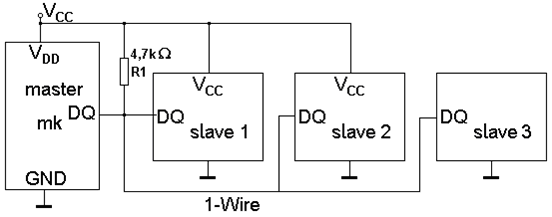
\includegraphics[scale=0.5]{1wire}
\caption{Schemat magistrali 1-Wire}
\label{fig:1wire}
\end{figure}

Magistrala, do poprawnego działania, wymaga rezystora podciągającego około 4,7~$\Omega$ do zasilania.
\chapter{Programowanie mikrokontrolerów ARM}

\section{Używanie bibliotek Linux'a}

\section{Środowisko programowania}
Kod programu oraz obsługi stacji pogody, zaimplementowanej na mikrokontrolerze BeagleBone black, został napisany przy użyciu środowiska programistycznego Eclipse. Środowisko to zostało wybreane przez wzgląd na ogromne możliwości, które ułatwiają w znacznej mierze programowanie oraz skracają jego czas. Eclipse jest darmowym narzędziem do programowania, jest intuicyjny w obsłudze, a przede wszystkim posiada wielką rzeszę użytkowników, przez co w przypadku problemów, ich rozwiązanie jest niemal natychmiastowe. Środowisko to można pobrać z oficjalnej strony, w projekcie został wykorzystany \emph{Eclipse IDE for C/C++ Developers}.

\begin{figure}[h]
\centering
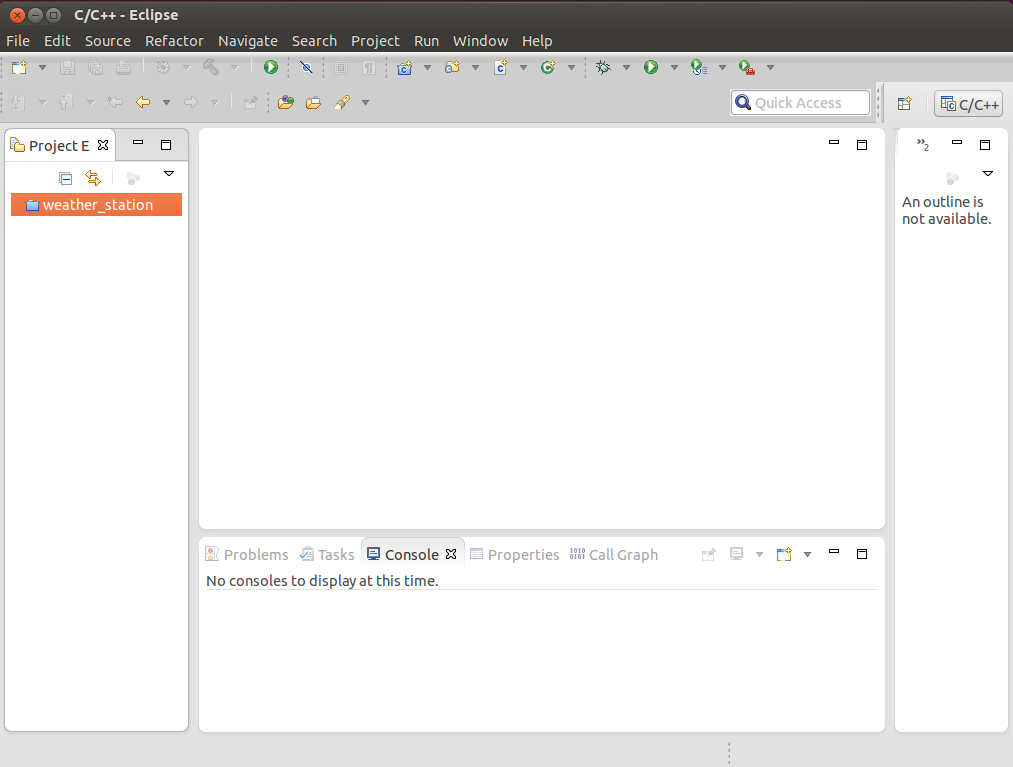
\includegraphics[scale=0.36]{eclipse}
\caption{Główny wygląd Eclipse'a}
\label{fig:eclipse}
\end{figure}

Po rozpakowaniu gotowego środowiska oraz jego uruchomieniu można już zacząć pracę z mikrokontrolerem, wystarczy jeszcze dokonać parę zabiegów, aby czas od zbudowania projektu, do jego uruchomienia na BeagleBone'ie była krótki. W celu uzyskania jak najwygodniejszej konfiguracji, został uruchomiony Eclipse na systemie operacyjnym Ubuntu, na którym były przechowywane wszystkie źródła. Dzięki odpowiedniemu dodatkowi do Eclipse'a - Remote System Explorer istnieje możliwość tworzenia programu na komputerze, jego cross-kompilacji do aplikacji wykonywalnej oraz uruchomienia gotowego pliku binarnego na mikrokontrolerze. Dzieje się to dzięki wspomnianemu wcześniej protokołowi SSH.

Aby stworzyć nowy projekt należy kliknąć File->New->C Project (może być również C++), pojawi się następujące okno:

\begin{figure}[h]
\centering
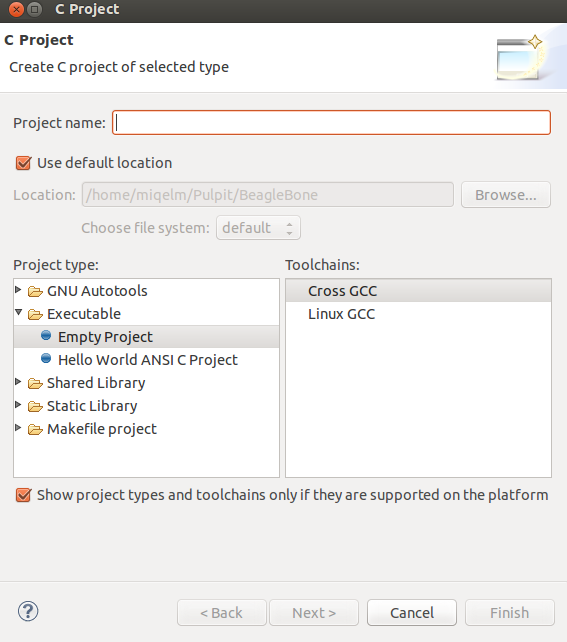
\includegraphics[scale=0.36]{eclipse_new}
\caption{Tworzenie nowego projektu}
\label{fig:eclipse_new}
\end{figure}

Po uzupełnieniu nazwy projektu oraz wyboru Cross GCC, przechodzimy dalej i kończymy konfigurację. Teraz następuje najważniejsza rzecz. Aby skompilować nasz projekt i móc go uruchomić na innej platformie sprzętowej, jaką jest procesor ARM, potrzebujemy cross-kompilatora. Jest to wymagane, gdyś komputer oraz BeagleBone różnią się budową oraz sposobem komunikacji na najniższym poziomie. W związku z tym, należy na komputerze zainstalować narzędzie umożliwiające nam generowanie pliku binarnego na inną platformę sprzętową, proces ten jest nazywany cross-kompilacją.

BeagleBone Black jest wyposażony w procesor o architekturze ARM hard float, dlatego też potrzebujemy do niego kompilatora, nazywa się on arm-linux-gnueabihf-gcc. Aby go zainstalować, należy w konsoli użytkownika wpisać następującą komendę:\newline
\emph{sudo apt-get install arm-linux-gnueabihf-gcc}\newline
Potwierdzająć chęć zainstalowania oraz pomyślnym przebiegu instalacji, jesteśmy w stanie teraz skompilować program na architekturę ARM.

W Eclipse klikając teraz prawym przyciskiem myszy na nowo stworzony projekcie, następnie wciśnięciu Properties, ukazują nam się właściwości projektu. Należy teraz zakomunikować środowisku, że program będzie kompilowany przy użyciu zainstalowanego przed chwilą kompilatora. W tym celu należy uruchomić zakładkę C/C++ Build, a potem opcję Settings i Cross GCC Compiler, w polu Command należy wpisać nazwę cross-kompilatora. Poniżej zostaje zamieszczony zrzut ekranu przedstawiający zaistniałą sytuację:

\begin{figure}[h]
\centering
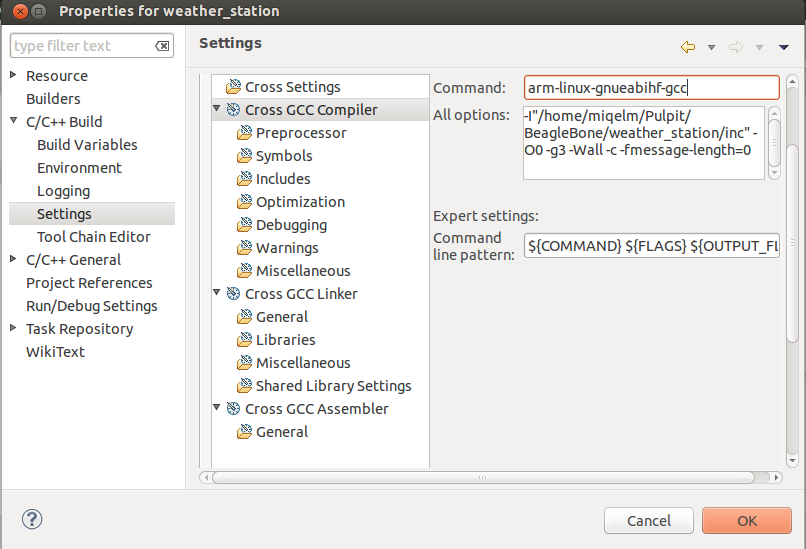
\includegraphics[scale=0.36]{eclipse-settings}
\caption{Ustawienia projektu}
\label{fig:eclipse-settings}
\end{figure}

W podobny sposób należy wypełnić również pola Command w zakładkach Cross GCC Linker oraz Cross GCC Assembler, ten ostatni należy wypełnić wpisując: arm-linux-gnueabihf-as.

\section{Kompilator}

\part{Wykorzystany sprzęt}
\chapter{Mikrokomputer BeagleBone Black}
Projekt inżynierski został zrealizowany, w głównej części, na mikrokomputerze BeagleBone Black. Został on stworzony specjalnie z myślą o programistach OpenSource oraz tych, dla których liczy się niskie zużycie energii. Jest to oparta na procesorze AM335x ARM Cortex-A8, taktowany częstotliwością 1 GHz, płytka developerska, która została wyposażona w 512 MB pamięci RAM, 2 GB pamięci FLASH, akcelerator grafiki 3D. Posiada szereg różnych interfejsów, takich jak: HDMI, USB, Ethernet, czytnik kart microSD. BeagleBone można zasilać na dwa sposoby, pierwszy - poprzez kabel USB podłączony do USB (5V) albo przy użyciu zewnętrznego zasilacza, również 5V. Dla użytkownika zostały również wyprowadzone 96 pinów typu wejśćie/wyjście.

Na mikrokomputerze można zainstalować i ze swobodą korzystać z najpopolarniejszych dystrybucji Linuxa, np. Ubuntu, Debian, Fedora, Arch. Istnieje również możliwość uruchomienia na BeagleBone systemu Android.


\chapter{Czujnik ciśnienia atmosferycznego BMP085}
\begin{figure}[h]
\centering
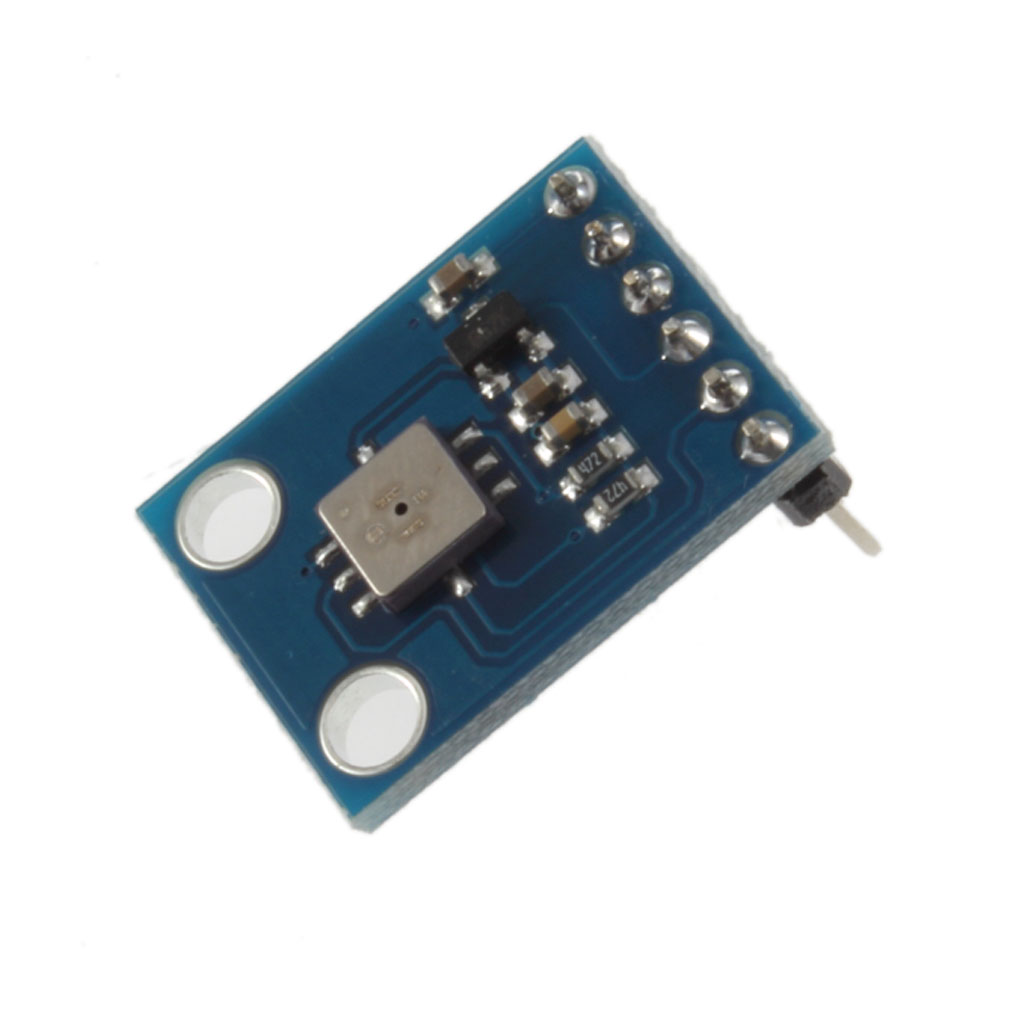
\includegraphics{bmp085_dol}
\caption{Czujnik ciśnienia BMP085 - widok z dołu}
\label{fig:bmp085_dol}
\end{figure}

\begin{figure}[h]
\centering
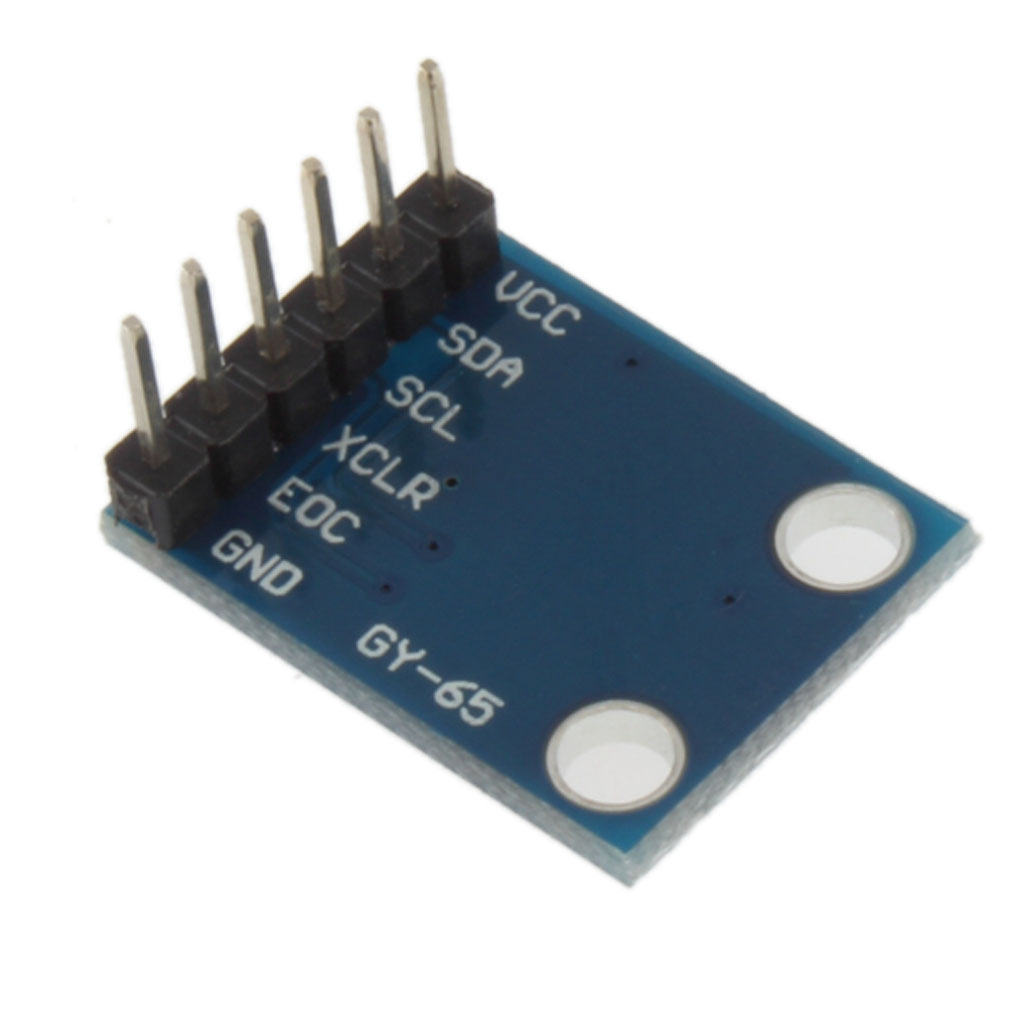
\includegraphics{bmp085_gora}
\caption{Czujnik ciśnienia BMP085 - widok z góry}
\label{fig:bmp085_gora}
\end{figure}
\chapter{Czujnik wilgotności DHT-22}
\section*{Opis}
DHT-22 jest cyfrowym oraz fabrycznie skalibrowanym czujnikiem względnej wilgotności i~temperatury. Został zbudowany w oparciu o 8 bitowy mikrokontroler, do którego podłączone są sensory. Małe rozmiary, stabliność pomiarowa, możliwość zainstalowania czujnika na duże odległości oraz niewielki pobór energii czyni go bardzo dobrym rozwiązaniem, nawet w ciężkich warunkach atmosferycznych.

Czujnik posiada swój własny sposób uzyskiwania pomiarów. Jest on podobny do magistrali szeregowej o nazwie 1-Wire. Do prawidłowego działania urządzenia potrzebne są dwa przewody zasilania oraz linia danych, poprzez którą następuje komunikacja. Należy również podłączyć do linii danych oraz zasilania rezystor podciągający o oporze około 3,3 k$\Omega$.
\section*{Dane charakterystyczne}
Jak podaje specyfikacja czujnika, może być on zasilany napięciem od 3,3 do 6 V. Posiada on następujące parametry: zakres mierzonej wilgotności od 0 do 100 \% (z dokładnością +-2\%) oraz temperatury od -40 do 80 stopni Celsjusza (z dokładnością +-0,5 stopnia).

Wygląd czujnika został przedstawiony na poniższym zdjęciu:
\begin{figure}[h]
\centering
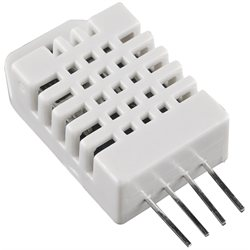
\includegraphics[scale=0.65]{dht22}
\caption{Czujnik wilgotności DHT-22}
\label{fig:dht22}
\end{figure}
\section*{Pobieranie danych z czujnika}
Zgodnie ze specyfikacją, załączoną do DHT-22, linia danych jest wolna, jeżeli jest na niej ustawiony stan wysoki. Czujnik, gdy nie jest używany, jest ustawiony w tryb spoczynku i niskiego poboru prądu. Poprzez wysłanie sygnału startu jest on wybudzany do trybu pracy i wysyła dane. Aby rozpocząć pomiar trzeba wysłać sygnał startu, należy to uczynić poprzez zwarcie do masy linii danych na conajmniej 1 ms. Po tym czasie czujnik zgłasza swoją obecność w układzie poprzez wystawienie logicznej jedynki na około 20-40 $\mu$s, następnie linia danych jest zwalniana oraz ponownie podciągana do zasilania, każda z tych czynności trwa 80 $\mu$s. Rysunek \ref{fig:inicjalizacja_dht} przedstawia inicjalizację czujnika DHT-22.
\begin{figure}[h]
\centering
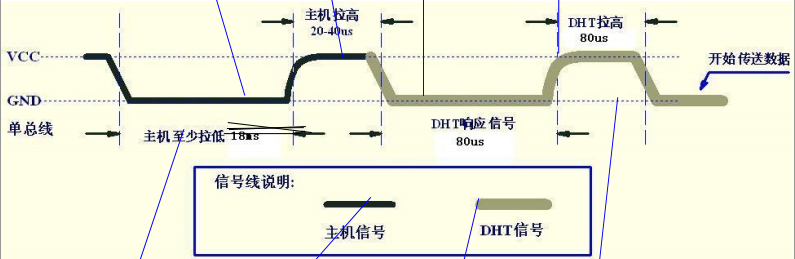
\includegraphics[scale=0.35]{inicjalizacja_dht}
\caption{Inicjalizacja czujnika}
\label{fig:inicjalizacja_dht}
\end{figure}
Po zgłoszeniu swojej obecności w układzie, czujnik zaczyna wysyłać 40 bitów danych, pierwsze 16 bitów odpowiada za ciśnienie, następne 16 to temperatura oraz końcowe 8 bitów służy jako suma kontrolna.

Aby przekonwertować odebrane dane na wskazania czujnika, należy obie liczby 16-bitowe, odpowiadające wilgotności oraz temperaturze, podzielić przez 10. W ten sposób otrzymujemy pomiary z dokładnością do jednego miejsca po przecinku. Po odebraniu danych należy przede wszystkim sprawdzić, czy to co zostało otrzymane jest prawidłowe. Należy pierwsze 4 bajty dodać do siebie oraz sprawdzić, czy 8 młodszych bitów tej wartości są równe ostatniemu odebranemu bajtowi. Jeżeli tak, procedura odebrania została zakończona sukcesem. W przeciwnym wypadku należy spróbować ponownie pobrać dane z czujnika. Próby odczytu należy wykonywać do momentu przekroczenia maksymalnej ich liczby, przez co można uniknąć nieskończonej liczby prób odczytu.

Sposób kodowania informacji na linii danych przez DHT-22 jest następujący: każda wartość logiczna (0 oraz 1) jest reprezentowana przez podpięcie linii do zasilania na ustaloną chwilę czasową. Bit o wartości 0 jest wysyłany jako wysoki poziom przez okres 26-28 $\mu$s, natomiast czas trwania sygnału wysokiego dla bitu 1 wynosci 70 $\mu$s. Pomiędzy nadaniem odpowiedniego bitu, występuje przerwa - podłączenie linii danych do poziomu masy na około 50 $\mu$s.

Przebiegi poniżej pokazują wysyłanie danych:
\begin{figure}[h]
\centering
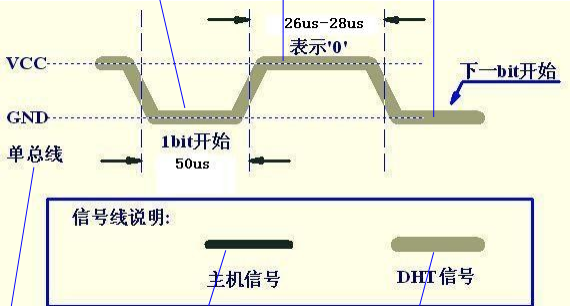
\includegraphics[scale=0.3]{zero_dht}
\caption{Wysłanie logicznego $"0"$}
\label{fig:zero_dht}
\end{figure}

\begin{figure}[h]
\centering
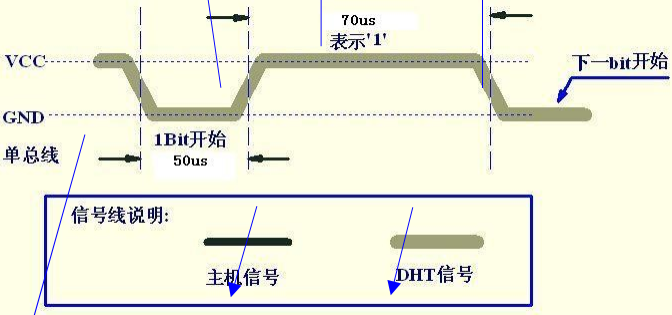
\includegraphics[scale=0.3]{jedynka_dht}
\caption{Wysłanie logicznej $"1"$}
\label{fig:jedynka_dht}
\end{figure}

Wysyłanie danych jest zakończone, jeżeli linia danych jest podłączona do zasilania oraz nie zmienia się jej stan. Czujnik wtedy przechodzi w stan uśpienia i będzie w nim przebywał aż do pojawienia się następnego sygnału startu. Jeżeli sygnał na linii danych jest zawsze w stanie wysokim, oznacza to niepoprawne działanie czujnika, może to być spowodowane wadliwym podłączeniem. 

\section*{Algorytm odczytu pomiarów}
Podczas odczytywania danych bardzo ważne są czasy występowania odpowiednich wartości logicznych. Błędna analiza czasu skutkuje złym zinterpretowaniem danych, co prowadzi do sfałszowania wyników.

Algorytm zastosowany przy tworzeniu pracy jest bardzo prosty. Polega on na odczytywaniu przy każdej możliwości stanu linii danych oraz zliczaniu liczby wystąpień stanu wysokiego, gdyż tylko ten koduje wysyłane wartości z czujnika.

Linia danych jest próbkowana do momentu odczytania 40 bitów. Jest ona ustawiana wówczas w stan wysoki, czujnik przechodzi w stan spoczynku. Po zakończeniu odczytu następuje analiza przetworzonych danych.

Liczba wystąpień każdego stanu wysokiego podlega procesowi podziału na dwa zbiory. Zadaniem tej funkcjonalności jest znalezienie odpowiedniej wartości granicznej, takiej która jednoznacznie określa ile razy musiał być spróbkowany sygnał na linii danych, aby został on zinterpretowany jako bit $"1"$ lub $"0"$. Zostało to zaimplementowane poprzez znalezienie minimalnej i maksymalnej wartości liczby wystąpień oraz wyliczniu średniej tych dwóch liczb, wynik tego działania był wartością progową przy dzieleniu na dwa zbiory, czyli binaryzacji.

Po wyliczeniu progu binaryzacji, liczba wystąpień została poddana porównaniu z nią, jeżeli była większa od progu, oznaczało to bit "1", w przeciwnym wypadku, było to kodowane jako "0".

Diagram pokazany na rysunku \ref{fig:diagram_dht22} przedstawia schemat blokowy algorytmu odczytu danych z czujnika DHT-22.
\begin{figure}[h]
\centering
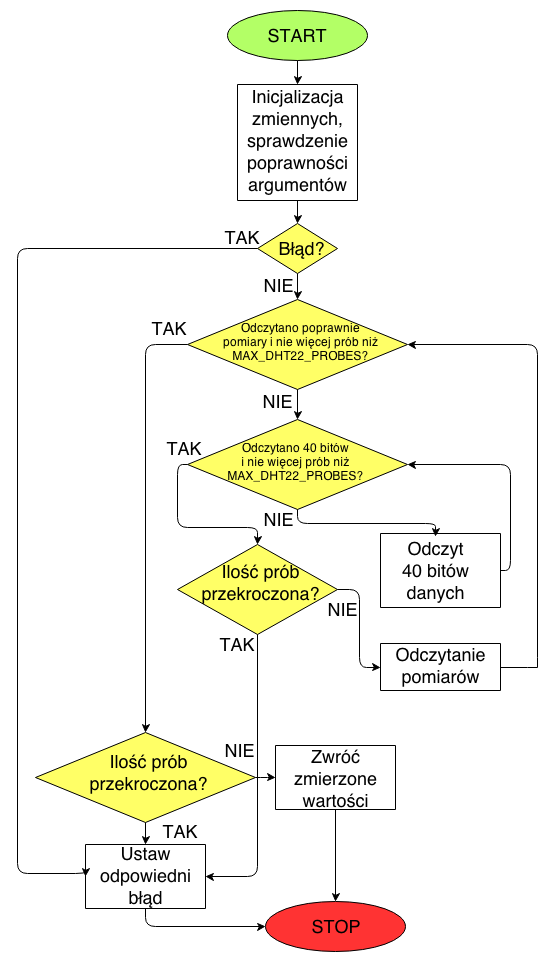
\includegraphics[scale=0.6]{diagram_dht22}
\caption{Diagram odczytu danych z czujnika DHT-22}
\label{fig:diagram_dht22}
\end{figure}

\part{Część praktyczna}



\chapter{Elektroniczny system pomiarów}
\chapter{Tworzenie aplikacji}
\chapter{Przechowywanie oraz wyświetlanie wyników}

\section{Baza danych MySQL}
Pomiary ze stworzonej stacji pogodowej zostają wysyłane nieustannie, w trakcie działania programu, do bazy danych MySQL. Znajduje się ona na serwerze AGH i została skonfigurowana poprzez stronę http://mysql.agh.edu.pl. Baza przechowuje wartości wszystkich zmierzonych parametrów meteorologicznych od pierwszego uruchomienia stacji pogody.

Struktura bazy danych jest prosta, posiada ona tabelę o nazwie "weather\_station". To właśnie w niej bezpośrednio przechowywane są wartości pomiarowe.

Składa się ona z sześciu kolumn:
\begin{enumerate}
\item godzina wykonania pomiaru i wysłania do bazy
\item data
\item temperatura z czujnika DHT-22
\item wilgotność z czujnika DHT-22
\item temperatura z czujnika BMP085
\item ciśnienie z czujnika BMP085
\end{enumerate}

\section{Strona internetowa z wynikami pomiarów}

\section{Interfejs użytkownika}
Strona internetowa, która została stworzona specjalnie do wizualizacji wyników ma bardzo prosty i intuicyjny interfejs użytkownika.

Główną jego częścią są ostatnie wskazania z czujników. Poniżej tych znajduje się wykres historii pomiarów każdego parametru. Wykres jest dowolnie konfigurowalny, użytkownik może wybrać, które wartości mają zostać pokazane, a które mają być ukryte. Dodatkowym udogodnieniem jest możliwość regulowania zakresem daty, w którym mają zostać pokazane pomiary.
\chapter{Rezultaty pomiarów}
Testy całego systemu pomiarowego zostały przeprowadzone w dwóch różnych środowiskach. W pierwszym przypadku mierzone były warunki atmosferyczne panujące na zewnątrz budynku mieszkalnego. Drugi test został przeprowadzony w warunkach mieszkalnych.
\section*{Warunki zewnętrzne}
Cały układ pomiarowy został testowo wykorzystany do badania warunków  meteorologicznych panujących na wolnym powietrzu. Aplikacja zbierająca dane została uruchomiona na kilka godzin (od około 15:00 do 21:00).

Poniższe wykresy prezentują warunki wtedy panujące. Jak widać na załączonych rysunkach, temperatura stale maleje wraz z upływem czasu. Świadczy to o poprawnym pomiarze, gdyż wraz z zachodzącym słońcem, robi się coraz chłodniej.
\begin{figure}[h!]
\centering
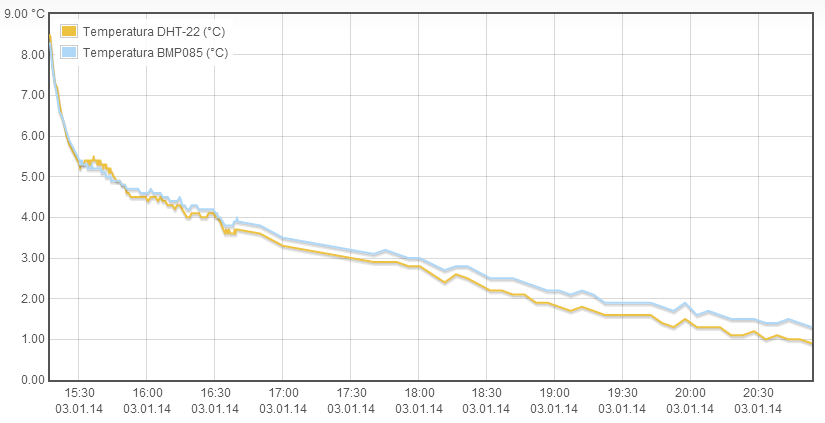
\includegraphics[scale=0.65]{zewnatrz_temp}
\caption{Pomiar temperatury na zewnątrz budynku}
\label{fig:zewnatrz_temp}
\end{figure}

Rysunek \ref{fig:zewnatrz_reszta} przedstawia zależności wilgotności powietrza oraz ciśnienia atmosferycznego od czasu, w którym następowało badanie.
\begin{figure}[h!]
\centering
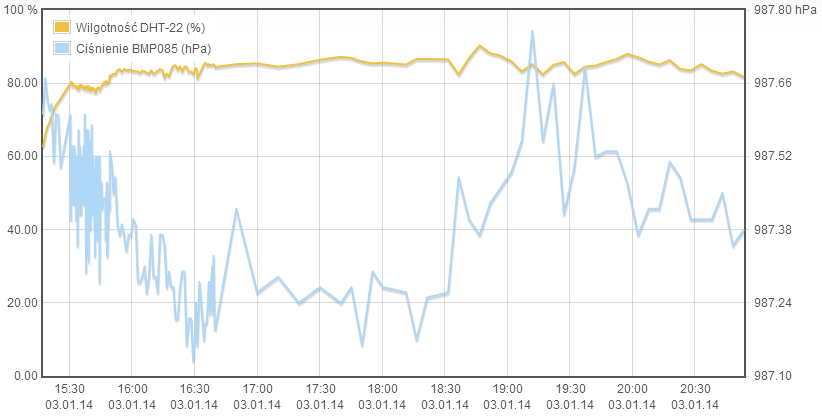
\includegraphics[scale=0.65]{zewnatrz_reszta}
\caption{Pomiar wilgotności oraz ciśnienia na zewnątrz budynku}
\label{fig:zewnatrz_reszta}
\end{figure}

Wahania ciśnienia atmosferycznego widoczne na wykresie \ref{fig:zewnatrz_temp} spowodowane są szumem występującym na czujniku oraz jego dokładnością.

\section*{Warunki pokojowe}
Następnie stacja pogodowa została ustawiona w pokoju, gdzie temperatura nie ulega dużym wahaniom i uruchomiono aplikacją zbierającą pomiary. Wykres na rysunku \ref{fig:wewnatrz_temp} przedstawia zależność temperatur od czasu, natomiast rysunek \ref{fig:wewnatrz_reszta} prezentuje pomiary ciśnienia atmosferycznego oraz wilgotności.
\begin{figure}[h!]
\centering
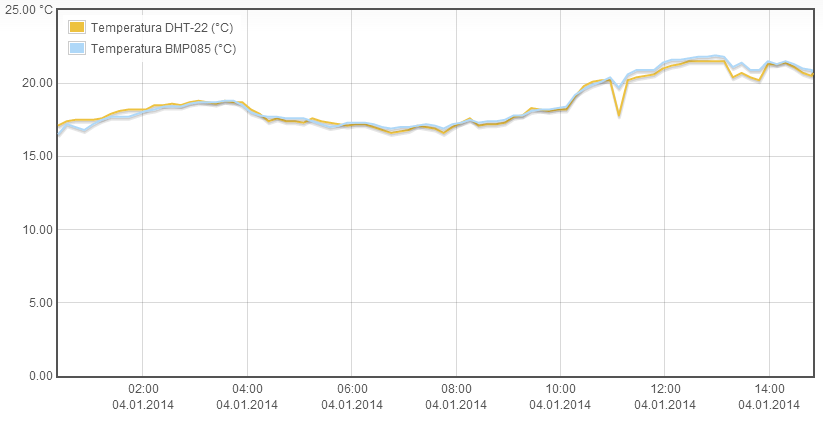
\includegraphics[scale=0.65]{wewnatrz_temp}
\caption{Pomiar temperatury wewnątrz pomieszczenia}
\label{fig:wewnatrz_temp}
\end{figure}
Jak można zauważyć z wykresu temperatur, w nocy miała ona stosunkowo niską wartość, natomiast nad ranem zaczeła rosnąć. Wiąże się to z faktem chłodzenia powietrza w nocy, w celu uzyskania lepszego wypoczynku podczas snu oraz zwiększenia poziomu ogrzewania na czas pracy.

\begin{figure}[h!]
\centering
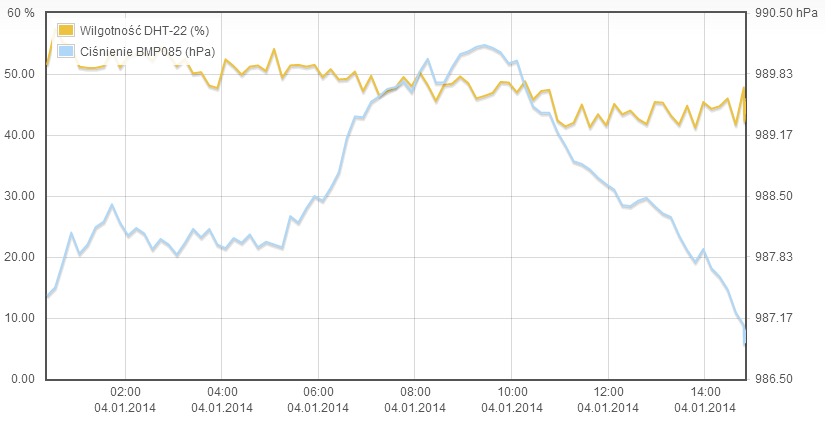
\includegraphics[scale=0.65]{wewnatrz_reszta}
\caption{Pomiar wilgotności oraz ciśnienia wewnątrz pomieszczenia}
\label{fig:wewnatrz_reszta}
\end{figure}
\chapter{Podsumowanie}
Projekt inżynierskii opisany w niniejszej pracy ma na celu badanie warunków meteorologicznych badając trzy pomiary: temperaturę, ciśnienie oraz wilgotność powietrza.

Testy przeprowadzone po ukończeniu tworzenia układu oraz oprogramowania dowodzą, że projekt inżynierski został zakończony sukcesem, wszystkie zaplanowane funkcjonalności zostały zrealizowane. Pomiary warunków meteorologicznych, które zostały zmierzone były bardzo zbliżone do wskazań otrzymanych przy pomocy standardowych urządzeń pomiarowych, jak np. termometr pokojowy.

Największym problemem napotkamym podczas tworzenia niniejszego projektu było doprowadzenie do kompilacji pełnego projektu, wraz ze wszystkimi bibliotekami, cross-kompilowaniem oraz uruchamianiem aplikacji na innej architekturze niż na tej, na której tworzone było oprogramowanie.

Możliwymi koncepcjami rozwinięcia tematyki niniejszej pracy dyplomowej jest stworzenie i uruchomienie algorytmów do przewidywania pogody. Jest to zagadanienie bardzo trudnie i~skomplikowanie, jednakże na pewno bardzo interesujące.

Inną możliwością jest zastosowanie mikrokomputera BeagleBone oraz czujnika ciśnienia atmosferycznego do zbudowania urządzenia pomiarowego, stosowanego w obiektach latających, np. kwadrokopter.
\addcontentsline{toc}{part}{Bibliografia}
\bibliographystyle{alpha}
\begin{thebibliography}{1}

\bibitem{bugusz}
Jacek Bogusz
\newblock {\em Lokalne interfejsy szeregowe w systemach cyfrowych}.
\newblock Wydawnictwo BTC, Warszawa, 2004.

\bibitem{mielczarek}
Wojciech Mielczarek
\newblock {\em Szeregowe interfejsy cyfrowe}.
\newblock Wydawnictwo HELION, Gliwice, 1993.

\bibitem{leonard}
Michael Leonard
\newblock {\em http://www.michaelhleonard.com/cross-compile-for-beaglebone-black/}.
\newblock [Dostęp: 11.12.2013].

\bibitem{wiki}
BeagleBone Black Wiki
\newblock {\em http://circuitco.com/support/index.php?title=BeagleBoneBlack}.
\newblock [Dostęp: 11.12.2013].

\bibitem{wiki}
Strona projektu ARM Hard Float
\newblock {\em http://www.armhf.com/}.
\newblock [Dostęp: 11.12.2013].

\bibitem{bmp085_spec}
Specyfikacja czujnika ciśnienia BMP085
\newblock {\em https://www.sparkfun.com/datasheets/Components/General/BST-BMP085-DS000-05.pdf}.
\newblock [Dostęp: 11.12.2013].

\bibitem{dht22_spec}
Specyfikacja czujnika ciśnienia DHT-22
\newblock {\em http://www.adafruit.com/datasheets/DHT22.pdf}.
\newblock [Dostęp: 11.12.2013].

\bibitem{php_mysql}
Luke Welling, Laura Thomson
\newblock {\em PHP i MySQL. Tworzenie stron WWW. Vademecum dla profesjonalisty. Wydanie czwarte.}.
\newblock Wydawnictwo HELION, Gliwice, 2009.

\bibitem{flot}
Strona główna projektu FlotChart
\newblock {\em http://www.flotcharts.org/}.
\newblock [Dostęp: 6.01.2014].

\bibitem{flot}
Strona główna środowiska programistycznego Eclipse
\newblock {\em http://www.eclipse.org/}.
\newblock [Dostęp: 6.01.2014].

\bibitem{flot}
Poradnik korzystania z MySQL C API
\newblock {\em http://zetcode.com/db/mysqlc/}.
\newblock [Dostęp: 6.01.2014].

\end{thebibliography}


% itd.
 \appendix
 \addcontentsline{toc}{part}{Załączniki}
\chapter{Kod źródłowy aplikacji}
% \include{dodatekB}
% itd.


\end{document}
